\documentclass[12pt]{article}
\title{ECE M16 Final}
\usepackage{subcaption}
\author{Lawrence Liu}
\usepackage{graphicx}
\usepackage[english,shorthands=off]{babel}        % shorhands=off is required for babel french in combination with tikz karnaugh....
\usepackage[utf8x]{inputenc}
\usepackage[T1]{fontenc}
\usepackage{amsmath}
\usepackage{geometry}
\geometry{verbose,a4paper, tmargin=3.5cm,bmargin=3.5cm,lmargin=2.5cm,rmargin=2.5cm,headsep=1cm,footskip=1.5cm}
\usepackage{colortbl}
\usepackage[dvipsnames]{xcolor}
\usepackage{tikz -timing}
\usepackage{tikz}
\usepackage{listings}
\usetikzlibrary{karnaugh}

\definecolor{LogisimKMapColor0}{RGB}{128,0,0}
\definecolor{LogisimKMapColor1}{RGB}{230,25,75}
\definecolor{LogisimKMapColor2}{RGB}{250,190,190}
\definecolor{LogisimKMapColor3}{RGB}{170,110,40}
\definecolor{LogisimKMapColor4}{RGB}{245,130,48}
\definecolor{LogisimKMapColor5}{RGB}{255,215,180}
\definecolor{LogisimKMapColor6}{RGB}{128,128,0}
\definecolor{LogisimKMapColor7}{RGB}{255,255,25}
\definecolor{LogisimKMapColor8}{RGB}{210,245,60}
\definecolor{LogisimKMapColor9}{RGB}{0,0,128}
\definecolor{LogisimKMapColor10}{RGB}{145,30,180}
\definecolor{LogisimKMapColor11}{RGB}{60,180,175}
\definecolor{LogisimKMapColor12}{RGB}{0,130,203}
\definecolor{LogisimKMapColor13}{RGB}{230,190,255}
\definecolor{LogisimKMapColor14}{RGB}{170,255,195}
\definecolor{LogisimKMapColor15}{RGB}{240,50,230}


\definecolor{codegreen}{rgb}{0,0.6,0}
\definecolor{codegray}{rgb}{0.5,0.5,0.5}
\definecolor{codepurple}{rgb}{0.58,0,0.82}
\definecolor{backcolour}{rgb}{0.95,0.95,0.92}

\lstdefinestyle{mystyle}{
    backgroundcolor=\color{backcolour},   
    commentstyle=\color{codegreen},
    keywordstyle=\color{magenta},
    numberstyle=\tiny\color{codegray},
    stringstyle=\color{codepurple},
    basicstyle=\ttfamily\footnotesize,
    breakatwhitespace=false,         
    breaklines=true,                 
    captionpos=b,                    
    keepspaces=true,                 
    numbers=left,                    
    numbersep=5pt,                  
    showspaces=false,                
    showstringspaces=false,
    showtabs=false,                  
    tabsize=2
}

\lstset{style=mystyle}

\begin{document}
\maketitle
\section*{Problem 1}
\begin{center}
\begin{tabular}{c| c c c c}
    & 1 & 1 & 0 & 1\\
    \cline{2-5}
    1 & 11 & 00 & 00 & 10 \\
    & 1 & & &\\
    \cline{2-2}
    101 & 10 & 00 & &\\
    & 1 & 01 & &\\
    \cline{2-3}
    1100 & & 11 & 00 &\\
    & & 0 & &\\
    \cline{3-4}
    & & 11 & 00 & 10\\
    11001 & & 1 & 10 & 01\\
    \cline{3-5}\\
    & & 1 & 10 & 01
    
\end{tabular}
\end{center}
\section*{Problem 2}
Basing on the assumption that $c[1:0]=11$ corresponds with $o[1:0]=i[1:0]$
we have that 
\begin{align*}
    a[1]&=\overline{c[1]}.\overline{c[0]}.i[7]+\overline{c[1]}.c[0].i[5]+
        c[1].\overline{c[0]}.i[3]+c[1].c[0].i[1]\\
        &=\overline{c[1]}.(\overline{c[0]}.i[7]+c[0].i[5])+c[1].(\overline{c[0]}.i[3]+c[0].i[1])
\end{align*}
\begin{align*}
    a[0]&=\overline{c[1]}.\overline{c[0]}.i[6]+\overline{c[1]}.c[0].i[4]+
        c[1].\overline{c[0]}.i[2]+c[1].c[0].i[0]\\
        &=\overline{c[1]}.(\overline{c[0]}.i[6]+c[0].i[4])+c[1].(\overline{c[0]}.i[2]+c[0].i[0])
\end{align*}
Which results in a circuit like this\\
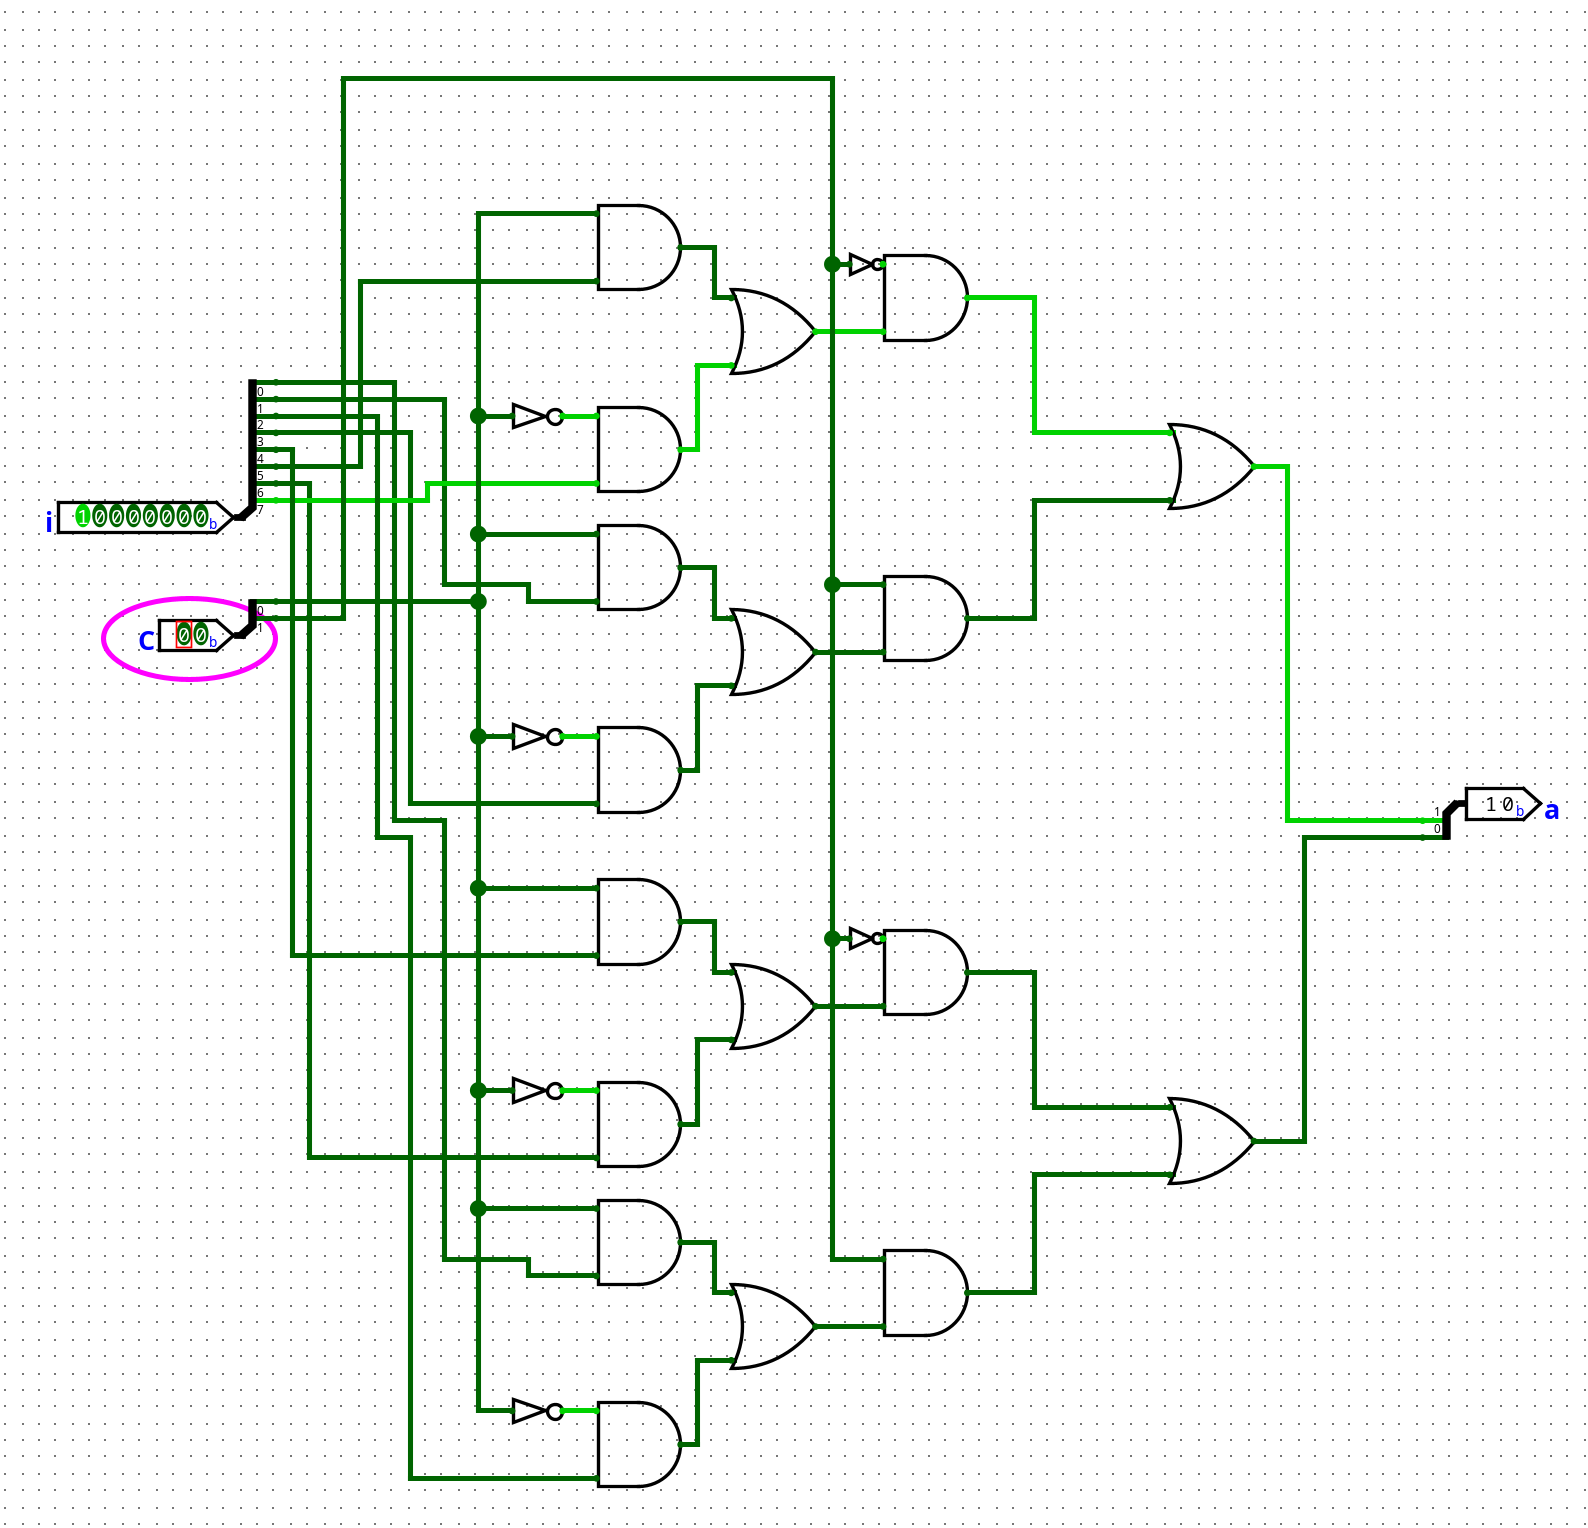
\includegraphics[scale=0.25]{fig1.png}
\section*{Problem 3}
I created the circuit, and it is shown above, and I tested it with the following python checker srcipt
\lstinputlisting[language=Python]{checker.py}
This script utilizes Logisim's command line ability. I had the files in the following format
\begin{verbatim}
ECEM16
 |- .gitignore
 |- Final
 | |- Logisim
 | | |- FinalQ3.circ
 | :
 | :
 | |- checker.py
 |- .gitignore
 |- logisim-evolution.jar
\end{verbatim}
\section*{Problem 4}
Let the output 
\end{document}
